\documentclass[12pt,letterpaper,fleqn]{article}
\usepackage{fullpage}
\usepackage[top=2cm, bottom=4.5cm, left=2.5cm, right=2.5cm]{geometry}
\usepackage{amsmath,amsthm,amsfonts,amssymb,amscd}
\usepackage[utf8]{inputenc}
\usepackage{lastpage}
\usepackage{enumerate}
\usepackage{fancyhdr}
\usepackage{mathrsfs}
\usepackage{xcolor}
\usepackage{graphicx}
\usepackage{listings}
\usepackage{hyperref}
\usepackage{amsmath}
\usepackage{nccmath}

\newcommand{\R}{\mathbb{R}}
\newcommand{\Q}{\mathbb{Q}}

\hypersetup{%
  colorlinks=true,
  linkcolor=blue,
  linkbordercolor={0 0 1}
}
 
\renewcommand\lstlistingname{Algorithm}
\renewcommand\lstlistlistingname{Algorithms}
\def\lstlistingautorefname{Alg.}

\lstdefinestyle{Python}{
    language        = Python,
    frame           = lines, 
    basicstyle      = \footnotesize,
    keywordstyle    = \color{blue},
    stringstyle     = \color{green},
    commentstyle    = \color{red}\ttfamily
}

\setlength{\parindent}{0.0in}
\setlength{\parskip}{0.05in}

% Edit these as appropriate
\newcommand\course{Física - Frente 2}
\newcommand\hwnumber{1}                  % <-- homework number
\newcommand\NetIDa{netid19823}           % <-- NetID of person #1
\newcommand\NetIDb{netid12038}           % <-- NetID of person #2 (Comment this line out for problem sets)

\pagestyle{fancyplain}
\headheight 35pt
%\lhead{\NetIDa}
%\lhead{\NetIDa\\\NetIDb}                 % <-- Comment this line out for problem sets (make sure you are person #1)
\chead{\textbf{\Large Elétrica - Circuitos \hwnumber}}
\rhead{\course \\ Junho/2019}
\lfoot{}
\cfoot{}
\rfoot{\small\thepage}
\headsep 1.5em

\begin{document}
    \begin{itemize}
        \item \textbf{Leis de Ohm, associação de resistores e corrente elétrica}
        \begin{enumerate}
            \item Encontre a resistência equivalente ($R_{eq}$) dos circuitos a seguir:
            \begin{enumerate}
                \item 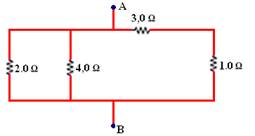
\includegraphics[]{circuito_1.jpg}
                \item 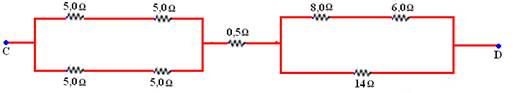
\includegraphics[]{circuito_2.jpg}
                \item 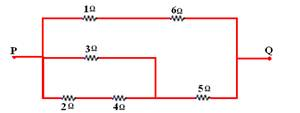
\includegraphics[]{circuito_3.jpg}
                \item 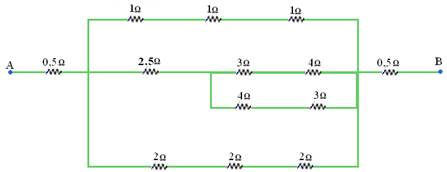
\includegraphics[]{circuito_4.jpg}
                \item 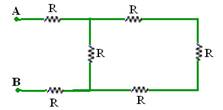
\includegraphics[]{circuito_5.jpg}
                \item 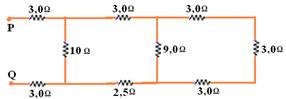
\includegraphics[]{circuito_6.jpg}
                \item 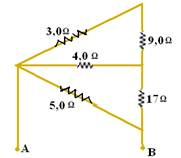
\includegraphics[]{circuito_7.jpg}
            \end{enumerate}
            
            \item \textbf{(UFMS/MS)} - No circuito elétrico abaixo, determine o valor da resistência equivalente entre os pontos A e B.
            
            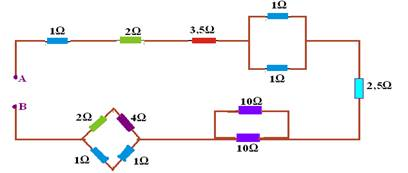
\includegraphics[]{circuito_ufms_1.jpg}
            
            \item \textbf{(MACKENZIE - SP)} - Uma caixa contém resistores conectados a três terminais, como mostra a figura abaixo.
            
            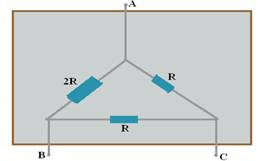
\includegraphics[]{circuito_mackenzie_6.jpg}
            
            A relação entre as resistências equivalentes entre os pontos A e B e entre os pontos B e C ($\frac{R_{AB}}{R_{AC}}$) 
            \begin{enumerate}
                \item 4/3
                \item 1
                \item 1/2
                \item 2/3
                \item 2
            \end{enumerate}
            
            \item \textbf{(CESGRANDERIO - RJ)} - No circuito abaixo, sabe-se que a resistência equivalente entre os pontos A e B vale 3$\Omega$.
            
            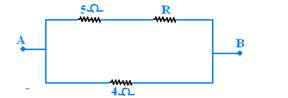
\includegraphics[]{circuito_cesgranderio_9.jpg}
            
            Então, o valor da resistência R, em ohms, deve ser igual a:
            \begin{enumerate}
                \item 3
                \item 4
                \item 5
                \item 6
                \item 7
            \end{enumerate}
            
            \item \textbf{(UFRN - RN)} - Um anel feito a partir de um fio condutor homogêneo possui, entre pontos diametralmente opostos, uma resistência R.
            
            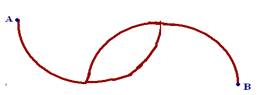
\includegraphics[]{circuito_ufrn_14.jpg}
            
            Se cortarmos esse anel em 4 partes iguais, duas a duas, tendo os pedaços maiores o dobro do comprimento dos pedaços menores, e os ligarmos como mostra a figura acima, podemos afirmar que, entre os pontos A e B, a resistência valerá: 
            
            \textit{Para esse exercício, lembre da $2^a$ Lei de Ohm $R = \frac{\rho l}{A}$, em que '$l$' é o comprimento do fio. Ou seja, quanto maior o fio, maior a resistência}
            
            \begin{enumerate}
                \item R/2 
                \item R/4
                \item R
                \item R/3
                \item 5R/2
            \end{enumerate}
            \pagebreak
            
            \item \textbf{(UFRJ - RJ)} - Um circuito é formado por uma bateria ideal, que mantém em seus terminais uma diferença de potencial V, um amperímetro ideal A, uma chave e três resistores idênticos, de resistência R cada um, dispostos como indica a figura. Com a chave fechada, o amperímetro registra a corrente I. Com a chave aberta, o amperímetro registra a corrente I’:
            
            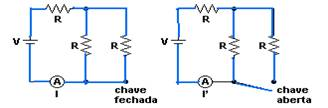
\includegraphics[]{circuitos_ufrj_16.jpg}
            
            \begin{enumerate}
                \item Calcule a razão I'/I;
                \item Se esses três resistores fossem usados para aquecimento da água de um chuveiro elétrico, indique se teríamos água mais quente com a chave aberta ou fechada. Justifique sua resposta.
            \end{enumerate}
            
            \item \textbf{(UFF-RJ)} - Em meados da primeira metade do século XIX, Georg Simon Ohm formulou uma lei que relaciona três grandezas importantes no estudo da eletricidade: tensão (V), intensidade de corrente (i) e resistência (R). Baseado nessa lei, a fim de verificar se um determinado resistor era ôhmico, um estudante reproduziu a experiência de Ohm, obtendo o seguinte gráfico:
            
            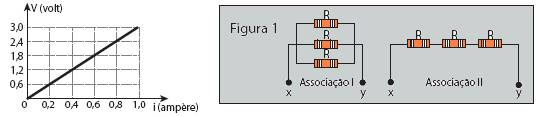
\includegraphics[]{grafico_uff_8.jpg}
            
            \begin{enumerate}
                \item Informe se o resistor utilizado na experiência do estudante é ôhmico e, em caso afirmativo, calcule o valor de sua resistência.
                \item Considere esse resistor submetido a uma tensão de 9,0 volts, durante um intervalo de tempo de 5,0 minutos, e determine, em joule, a energia dissipada.
                \item Repetindo a experiência com diversos resistores, o estudante encontrou um conjunto de três resistores ôhmicos idênticos e os associou de duas maneiras distintas, conforme representado na figura 1. O estudante, então, imergiu cada associação em iguais quantidades de água e submeteu seus terminais (X e Y) a uma mesma diferença de potencial, mantendo-a constante. Identifique, nesse caso, a associação capaz de aquecer, mais rapidamente, a água. Justifique sua resposta.
            \end{enumerate}
            \item \textbf{(PUC-RIO-2007)} - Ao aplicarmos uma diferença de potencial de 9,0 V em um resistor de 3,0 $\Omega$, podemos dizer que a corrente elétrica fluindo pelo resistor e a potência dissipada, respectivamente, são:
            
            \begin{enumerate}
                \item 1,0 A e 9,0 W 
                \item 2,0 A e 18,0 W
                \item 3,0 A e 27,0 W
                \item 4,0 A e 36,0 W
                \item 5,0 A e 45,0 W
            \end{enumerate}
            \item \textbf{(UFMG - 2010)} - Um professor pediu a seus alunos que ligassem uma lâmpada a uma pilha com um pedaço de fio de cobre. Nestas figuras, estão representadas as montagens feitas por quatro estudantes:
            
            \begin{figure}[h]
                \centering
                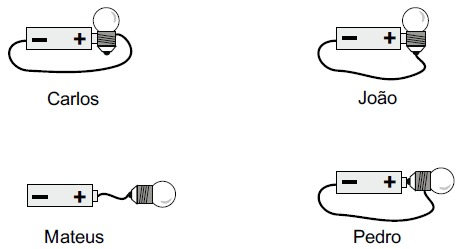
\includegraphics[width=0.5\textwidth]{montagem_ufmg_5_site_2.jpg}
            \end{figure}

            Considerando-se essas quatro ligações, é correto afirmar que a lâmpada vai acender apenas:
            \begin{enumerate}
                \item Montagem do Mateus  
                \item Montagem do João
                \item Montagem do João e do Pedro
                \item Montagem do Carlos, João e do Pedro
            \end{enumerate}
            \item \textbf{(UFF-2008)} - Em residências antigas, era comum que todos os eletrodomésticos fossem ligados a um único circuito elétrico, em geral montado com fios de ligação finos. Um modelo deste tipo de circuito está esquematizado na figura ao lado, onde r representa a resistência total dos fios de ligação. 
            Ao ligar eletrodomésticos com resistência baixa, como chuveiros elétricos, percebia-se uma diminuição no brilho das lâmpadas. Marque a alternativa que justifica tal diminuição no brilho das lâmpadas.
            
            \pagebreak
            \begin{figure} [h]
                \centering
                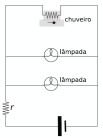
\includegraphics{circuit_uff_7_site_2.jpg}
            \end{figure}
            
            \begin{enumerate}
                \item 	A corrente total no circuito diminui, fazendo com que a diferença de potencial (ddp) aplicada às lâmpadas diminua e, portanto, a corrente através delas seja menor.
                \item Embora a diferença de potencial (ddp) nas lâmpadas permaneça a mesma, a corrente total no circuito diminui, diminuindo assim a corrente nas lâmpadas.
                \item A corrente total no circuito permanece a mesma mas, como a maior parte dela passa através do chuveiro, sobra menos corrente para as lâmpadas.
                \item A corrente total no circuito aumenta, aumentando assim a resistência das lâmpadas, o que diminui a corrente através delas.
                \item A corrente total no circuito aumenta, causando maior queda de potencial através de r e diminuindo assim a diferença de potencial (ddp) e a corrente nas lâmpadas.
            \end{enumerate}
            \item \textbf{(PUC-RJ)} - Duas resistências elétricas, uma de 2$\Omega$ e outra de 6$\Omega$, devem ser ligadas a uma bateria ideal de 12 V em um circuito elétrico.
            
            \begin{enumerate}
                \item Determine de que maneira as resistências devem ser ligadas para que a potência dissipada pelo circuito seja a menor possível.
                \item Desenhe o circuito correspondente à resposta do item a. 
                \item Determine o valor de tensão para o qual a bateria deveria ser ajustada de forma que a potência no circuito elétrico aumente em 300\%.
            \end{enumerate}
            \item \textbf{(FUVEST - SP)} - Considere um circuito formado por 4 resistores iguais, interligados por fios perfeitamente condutores. Cada resistor tem resistência R e ocupa uma das arestas de um cubo, como mostra a figura.
            
            \pagebreak
            \begin{figure}[h]
                \centering
                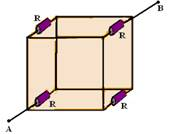
\includegraphics[]{circuito_fuvest_32.jpg}
            \end{figure}
            
            Aplicando entre os pontos A e B uma diferença de potencial U, a corrente que circulará entre A e B valerá:
            \begin{enumerate}
                \item 4U/R
                \item 2U/R
                \item U/R
                \item U/2R
                \item U/4R
            \end{enumerate}
            
            \item \textbf{(UEL - PR)} - No circuito elétrico, representado abaixo, os cinco resistores  apresentam a mesma resistência elétrica R. Calcule a resistência do resistor equivalente.
            
            \begin{figure}[h]
                \centering
                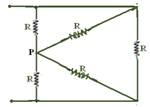
\includegraphics{circuito_uel_36.jpg}
            \end{figure}
            
            \item \textbf{(CEFET-MG)} - Dois resistores de 2,0 $\Omega$ e 4,0 $\Omega$ são ligados em série e, em seguida, o conjunto é conectado em paralelo a um resistor de 12 $\Omega$. A resistência equivalente dessa associação, em $\Omega$, é:
            
            \begin{enumerate}
                \item 2,0
                \item 4,0
                \item 8,0
                \item 12,0
                \item 16,0
            \end{enumerate}
            
            \pagebreak
            \item \textbf{(IME-RJ)} - Sabendo que todos os resistores da malha infinita da figura têm resistência R, a resistência equivalente entre A e B é:
            
            \begin{figure}[h]
                \centering
                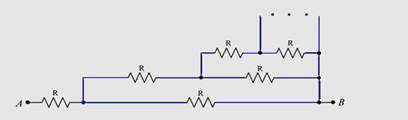
\includegraphics{circuito_ime_44.jpg}
            \end{figure}
            
            \begin{enumerate}
                \item $\frac{R(1+\sqrt{2})}{2}$
                \item $\frac{R(1+\sqrt{3})}{2}$
                \item $\frac{3R}{2}$
                \item $\frac{R(1+\sqrt{5})}{2}$
                \item $\frac{R(1+\sqrt{6})}{2}$
            \end{enumerate}
        \end{enumerate}
        \item \textbf{Ponte de Wheatstone}
        
        Charles Wheatstone montou um tipo de circuito elétrico em que é possível determinar a resistência de um componente elétrico desconhecido por meio de outras 3 resistências conhecidas e um galvanômetro (\textit{outro nome para amperímetro}). O circuito é montado da seguinte forma:
        \begin{figure}[h]
            \centering
            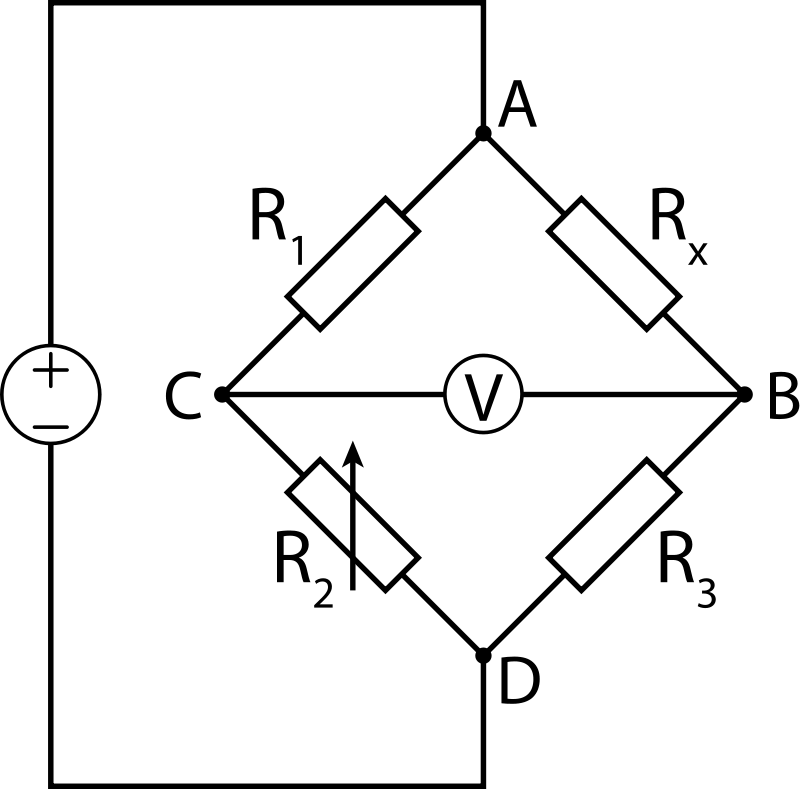
\includegraphics[width=0.3\textwidth]{ponte_wheatstone.png}
            \caption{Esquema do circuito elétrico, em que $R_1$, $R_2$ e $R_3$ são resistências conhecidas, um galvanômetro no meio da ponte e quer se determinar a resistência $R_x$}
            \label{fig:wheat_bridge}
        \end{figure}
        
        A ponte é dita \textbf{em equilíbrio} quando o galvanômetro não mede corrente passando. Em equilíbrio, a resistência desconhecida ($R_x$) é determinada pela relação:
        \begin{equation} \label{eq:ponte_wheatstone}
            \frac{R_1}{R_2} = \frac{R_3}{R_x}
        \end{equation}
        
        \begin{enumerate}
            \item Encontre o valor da resistência desconhecida ($R$), sabendo que o galvanômetro mede $i=0$.
            \begin{enumerate}
                \item 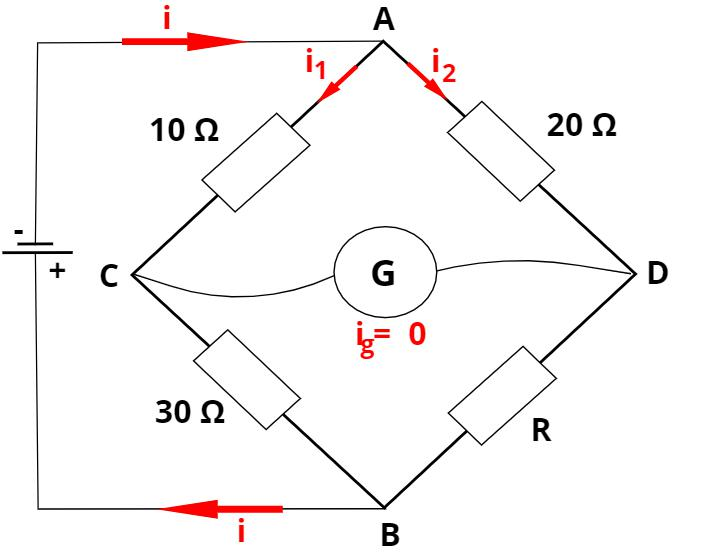
\includegraphics[width=0.3\textwidth]{ponte-de-wheatstone-exercicio-1.jpg}
                \item 
                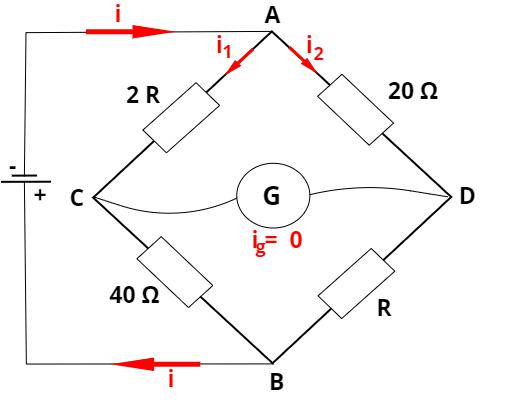
\includegraphics[width=0.3\textwidth]{ponte-de-wheatstone-exercicio-2.jpg}
            \end{enumerate}
            \item \textbf{(UFLA-MG)} - A ponte de Wheatstone mostrada abaixo estará em equilíbrio quando o galvanômetro G indicar zero volt. Para que isso ocorra, R1 deve ter valor igual a:
            
            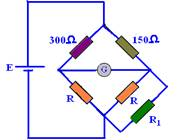
\includegraphics[width=0.3\textwidth]{ponte-de-wheatstone-ufla-11.jpg}
            \begin{enumerate}
                \item R/3
                \item R
                \item 2R
                \item R$^2$/2
                \item R$^2$
            \end{enumerate}
            \pagebreak
            \item \textbf{(UNICAMP)} - A variação de uma resistência elétrica com a temperatura pode ser utilizada para medir a temperatura de um corpo. Considere uma resistência R que varia com a temperatura $\theta$  de acordo com a expressão:
            $R=R_0(1+\alpha\theta)$, em que $R_0 = 1000 \Omega$, $\alpha = 4*10^{-3} \: ^{\circ}C^{-1}$ e $\theta$ é a temperatura em graus Celsius ($^{\circ}C$).
            Esta resistência está em equilíbrio térmico com o corpo, cuja temperatura $\theta$ se deseja conhecer. Para medir o valor de $R$, ajusta-se a resistência $R_2$, indicada no circuito abaixo, até que a corrente medida pelo amperímetro no trecho AB seja nula.
            
            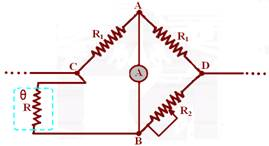
\includegraphics[width=0.5\textwidth]{ponte-de-wheatstone-unicamp-13.jpg}
            
            \begin{enumerate}
                \item Qual a temperatura $\theta$ do corpo quando a resistência $R_2$ for igual a 108 $\Omega$?
                \item A corrente através da resistência R é igual a $5,0.10^{-3} \:A$. Qual a diferença de potencial entre os pontos C e D indicados na figura?
            \end{enumerate}

            \item \textbf{(MACKENZIE-SP)} - No circuito a seguir, a ddp entre os terminais A e B é de 60V e o galvanômetro G acusa uma intensidade de corrente elétrica zero. Se a ddp entre os terminais A e B for duplicada e o galvanômetro continuar acusando zero, poderemos afirmar que:
            
            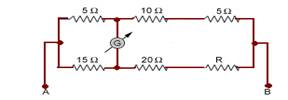
\includegraphics[width=0.5\textwidth]{ponte-de-wheatstone-mack-21.jpg}
            
            \begin{enumerate}
                \item a resistência R permanecerá constante e igual a 25 $\Omega$. 
                \item a resistência R permanecerá constante e igual a 15 $\Omega$.
                \item a resistência R permanecerá constante e igual a 10 $\Omega$.
                \item a resistência R permanecerá constante e igual a 50 $\Omega$.
                \item a resistência R permanecerá constante e igual a 12,5 $\Omega$.
            \end{enumerate}
        \end{enumerate}
    \end{itemize}
    \pagebreak
    \section*{Gabarito}
    \begin{itemize}
        \item \textbf{Leis de Ohm, associação de resistores e corrente elétrica}
        
        \begin{enumerate}
            \item 
            \begin{enumerate}
                \item $R_{eq}= 1 \Omega$
                \item $R_{eq}= 12,5 \Omega$
                \item $R_{eq}= 3,5 \Omega$
                \item $R_{eq}= 2,5 \Omega$
                \item $R_{eq}= 3R/2 $
                \item $R_{eq}= 11 \Omega$
                \item $R_{eq}= 4 \Omega$
            \end{enumerate}
            \item $R_{eq}= 16 \Omega$
            \item (a)
            \item (e)
            \item (e)
            \item \begin{enumerate}
                \item $\frac{i'}{i}=0.75$
                \item Com a chave fechada, pois a corrente elétrica é maior e como a potência elétrica é $P=Ui$, maior será a potência do chuveiro e mais quente será a água.
            \end{enumerate}
            \item \begin{enumerate}
                \item Sim, é ôhmico, pois o gráfico Vxi é linear e passa pela origem, o que leva a expressão $V=Ri$. A resistência ($R$), pelo gráfico é: $R=\frac{V}{i}=\frac{0.6}{0.2}= 3\Omega$
                \item $5\: min\: \implies\: 300s$. Sabemos que a forma da potência é dada por: $P=\frac{V^2}{R}$ e $P=\frac{E}{\Delta t}$. 
                
                Então: $\frac{E}{\Delta t}= \frac{V^2}{R} \implies E =\frac{V^{2}\Delta t}{R}$.  Como os dados do enunciado e do item (a) são: $V=9,0\:V$ e $R=3\: \Omega$. Então: $E=\frac{9^2*300}{3}= 8100 \:J$
                
                \item A Associação I é a capaz de aquecer a água mais rapidamente, pois a resistência equivalente ($R_{eq} = R/3$) é menor que a associação II ($R_{eq}=3R$) e, como a potência elétrica ($P$) é inversamente proporcional à resistência ($R_{eq}$ nesse caso), então a potência elétrica dissipada será maior.
            \end{enumerate}
            \item (c)
            \item (c)
            \item (e)
            \item \begin{enumerate}
                \item Como a potência é dada por $P=\frac{U^2}{R}$, quanto maior a resistência, menor é a potência. A associação que dá uma resistência equivalente maior possível é quando \textbf{as resistências estão em série.};
                \item \textit{Desenho com uma fonte e as duas resistências infileiradas}
                \item Um aumento de potência em 300\% significa que a potência, agora, é $4P$. Como a potência é proporcional ao quadrado da tensão ($P = \frac{U^2}{R_{eq}}$) e se $P \rightarrow 4P$, então $U \rightarrow 2U$. 
                Logo: $U_{novo}=2*12 = 24 V$
            \end{enumerate}
            \item Veja na figura abaixo, que os 4 resistores estão em curto circuito:
            
            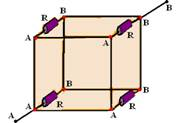
\includegraphics[width=0.4\textwidth]{sol_fuvest_32.jpg}
            
            Então, essa configuração equivale a um circuito com 4 resistores em paralelo. Então $R_{eq}= R/4$. Aplicando a Lei de Ohm , isolando a corrente elétrica: $i=U/R_{eq} = 4U/R$. Resposta: (a)
            
            \item $R_{eq}=R/2$
            \item (b)
            \item Vamos chamar de $R_{eq}$ toda a parte superior do circuito, de forma que a resistência entre A e B é:
            
            $R_{AB}= R + \frac{R*R_{eq}}{R+R_{eq}}$.
            
            Como a malha de resistência vai até o infinito, então a resistência entre A e B ($R_{AB}$) é basicamente a resistência da malha ($R_{eq}$). Logo, $R_{AB}=R_{eq}$.
            
            Portanto: $R_{AB}= R + \frac{R*R_{AB}}{R+R_{AB}} \implies R_{AB}(R+R_{AB})=R(R+R_{AB})+R*R_{AB}$.
            
            $R^2_{AB} - R*R_{AB}-R^2 = 0$
            
            Solucionando para $R_{AB}$ e levando em conta que não existe resistência negativa ($R_{AB}\nless0$): $R_{AB}=\frac{1+\sqrt{5}}{2}$. Resposta: (d)
        \end{enumerate}
        \item \textbf{Ponte de Wheatstone}
        \begin{enumerate}
            \item 
            \begin{enumerate}
                \item $R=60 \Omega$
                \item $R=20 \Omega$
            \end{enumerate}
            \item (b)
            \item \begin{enumerate}
                \item A fórmula para Ponte de Wheatstone em equilíbrio é: 
                
                $\frac{R_1}{R}=\frac{R_1}{R_2} \implies R=R_2=108 \Omega$.
                
                Logo, pela fórmula dada no enunciado:
                
                $108=100(1+4.10^{-3}\theta) \implies 1,08 = 1 +4.10^{-3}\theta$
                
                Portanto:$4.10^{-3}\theta= 0,08=8.10^{-2} \implies \theta = 20 ^{\circ}C$
                
                \item Como $R=R_2=108 \Omega$, então: $U=Ri \implies U=108*5.10^{-3}= 1,08 \: V$
            \end{enumerate}
            \item (a)
        \end{enumerate}
    \end{itemize}
\end{document}
